\section{Semaine 5 - 11 mars}

\subsection{Lundi - Masques}

L'\textbf{objectif} d'aujourd'hui est de créer de masques
pour que Victor puisse passer en salle blanche la semaine
prochaine. Les masques son celles qu'on a utilisé à la
session de nanofabrication. 

Nous allons créer les masques avec le logiciel 
\textsc{Layout Editor 3D}, avec les données que 
nous avons obtenu la semaine dernière en optimisant
la vraie bowtie.

\begin{figure}[h!]
    \centering
    \begin{subfigure}[b]{0.4\textwidth}
        \centering
        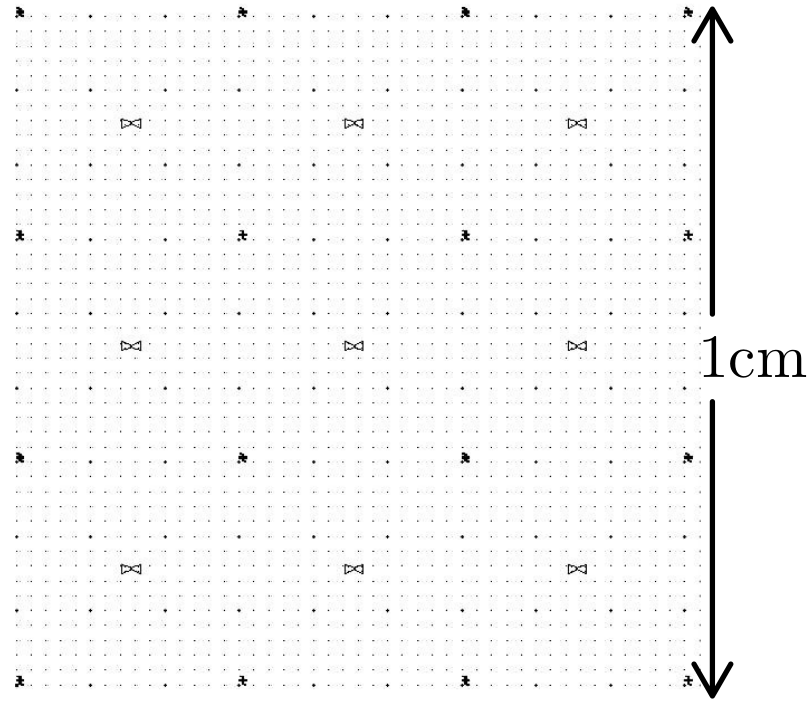
\includegraphics[width=0.8\linewidth]{texfigures/waffer.png}
        \caption{\label{fig:waffer} Masque de tout le waffer.}
    \end{subfigure}
    \begin{subfigure}[b]{0.4\textwidth}
        \centering
        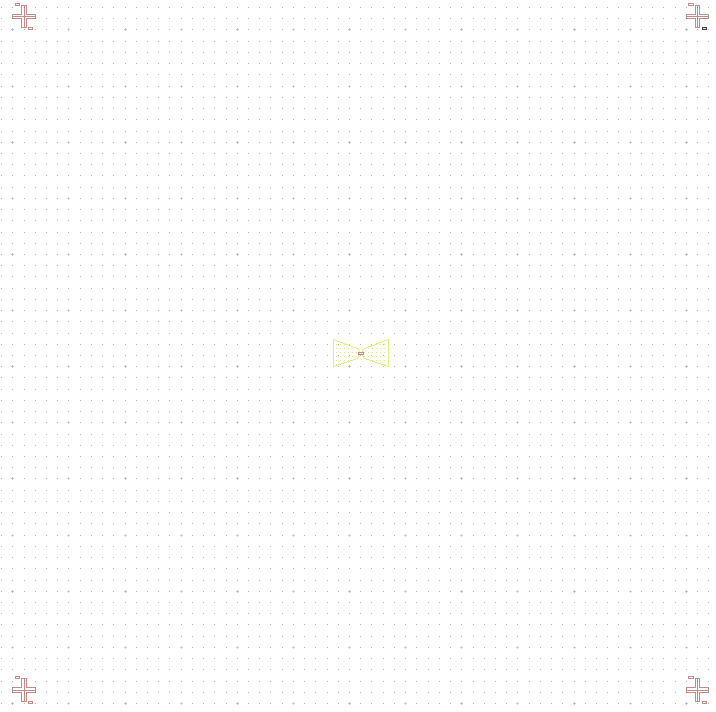
\includegraphics[width=0.8\linewidth]{texfigures/waffer_cell.png}
        \caption{\label{fig:waffer_cell} Zoom sur une cellule du waffer}
    \end{subfigure}
    \caption{Masque pour la nanofabrication.}
\end{figure}

\begin{figure}[h!]
    \centering
    \begin{subfigure}[b]{0.4\textwidth}
        \centering
        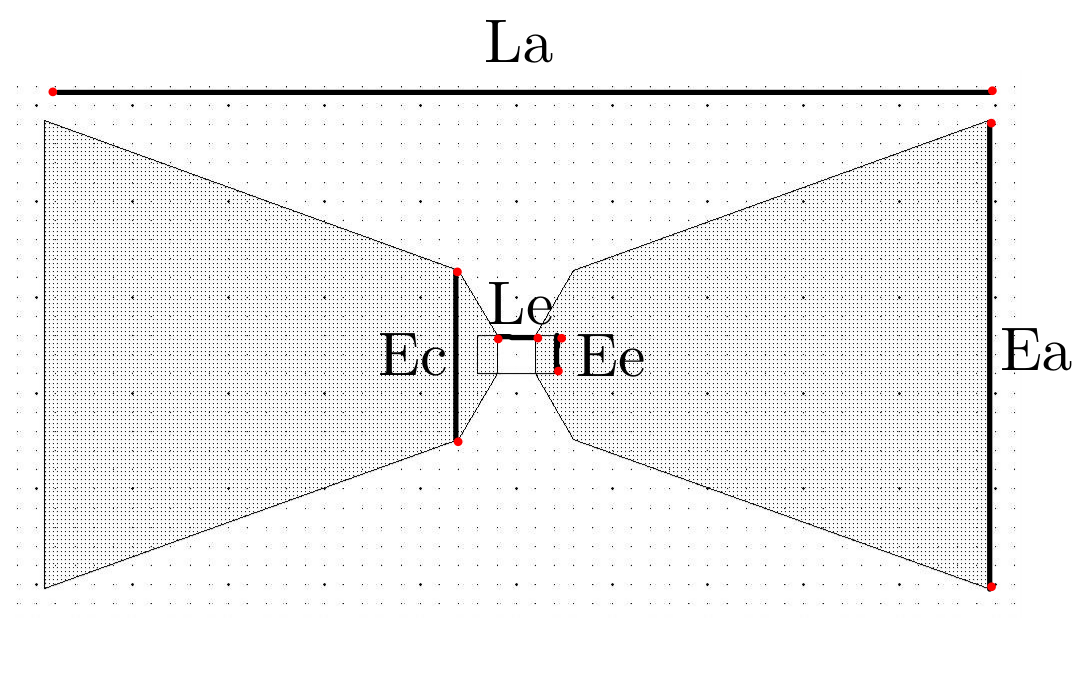
\includegraphics[width=0.8\linewidth]{texfigures/waffer_bowtie.png}
        \caption{\label{fig:waffer_bowtie} Zoom sur la bowtie.}
    \end{subfigure}
    \begin{subfigure}[b]{0.4\textwidth}
        \centering
        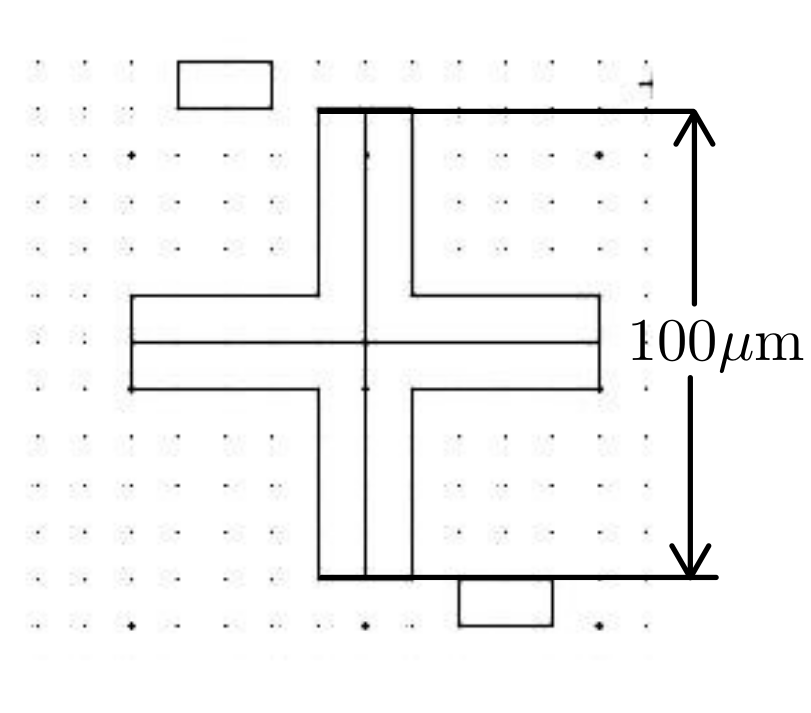
\includegraphics[width=0.8\linewidth]{texfigures/waffer_cross.png}
        \caption{\label{fig:waffer_cross} Zoom sur une croix d'alignement.}
    \end{subfigure}
    \caption{Zoom sur la masque.}
\end{figure}

\subsection{Mardi - Ondes planes}

L'\textbf{objectif} d'aujourd'hui sera d'expérimenter
avec les ondes planes.

La Figure \ref{fig:onde_plane} montre un schéma de la situation
à laquelle nous nous intéressons.

\begin{figure}[h!]
    \centering
    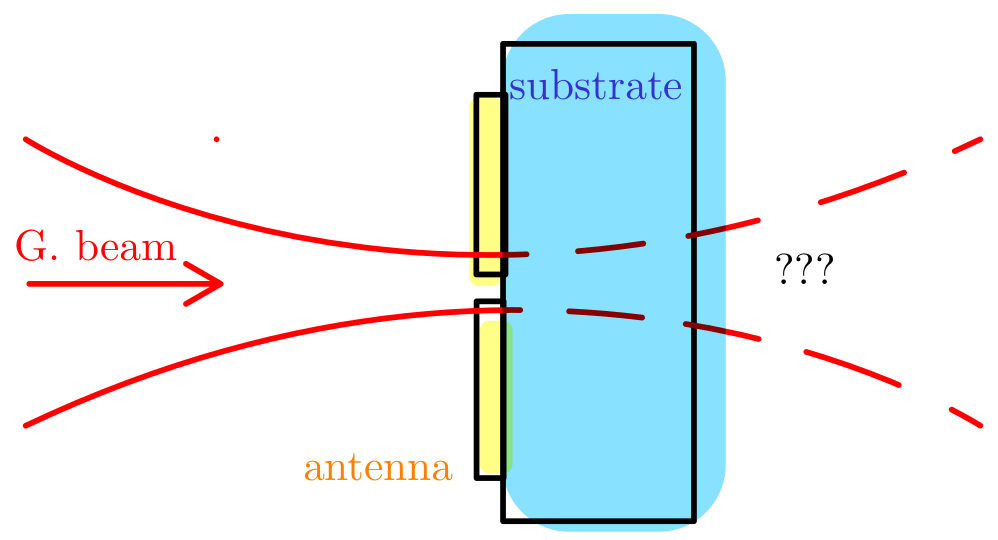
\includegraphics[width=0.5\textwidth]{texfigures/onde_plane.png}
    \caption{\label{fig:onde_plane} L'antenne est irradiée par un laser (un faisceau gaussien). Nous nous intéressons au champ transmis.}
\end{figure}


Jusqu'à maintenant, on a utilisé le S-parameters pour étudier nos
simulations. Cependant, le S-parameter n'est pas disponible
quand on travaille avec une onde plane au lieu d'avec un port.


Je pense que à chaque fois qu'on nous
demande d'expérimenter avec CST nous avons deux obstacles.
D'abord, nous ne sommes pas assez familiarisés avec le logiciel,
ensuite, j'ai plusieurs trous dans mes connaissances par rapport
à ce que nous sommes en train de faire.  Déjà, c'est 

